\section{Contexto}
Problemas de NP-difícil\cite{wiki:np-haardness} como os de empacotamento são problemas que já possuem grande bibliografia, onde métodos de simplificar a complexidade deles tendem a se limitar a formas geométricas simples como retângulos, tanto para os objetos quanto para a região de empacotamento. De forma que foi decidido analisar algoritmos que empacotem polígonos de diversas formas
geométricas, sobre uma bandeja, que também pode adquirir diversas formas.\newline

\cite{book:genetic_algo_data_structure}Os algoritmos genéticos possuem um longo histórico de encontrar bons resultados
por métodos que seriam exigidos força bruta ou um algoritmo de grande complexidade de tempo, os tornando um dos melhores candidatos para essa analise.

% Antes de se trabalhar com o empacotamento tridimensional em si, 
% é necessário obter os dados do objeto, como vértices e arestas. Para depois se 
% realizar o pre processamento dos objetos os tornando formas geométricas mais simples de se trabalha.

% \section{\textit{Mixed-Interger Linear Programming}}

% MILP é um dos algoritmos mais comuns para resolver o problema de empacotamento bidimensional,
% mas para poder ser utilizado, este algoritmo requer retângulos como forma geométricas para todos os objetos e
% para a região que se busca minimizar a areá.

% O MILP é um algoritmo para resolver problemas de otimização onde as restrições
% são um conjunto de inequações que podem ser simplificadas em inequações lineares ao substituir as variáveis de valor inteiro em um dos valores do seu conjunto, sendo este método chamado de \textit{LP relaxation}. Como no problema de maximação abaixo:

% \begin{equation}
% \label{eq:Cap01_MILP_Objective}
% \begin{aligned}
%  maxZ = 8x + 3y
% \end{aligned}
% \end{equation}
% \begin{equation}
% \label{eq:Cap01_MILP_01_Ineq_Integer01}
% \begin{aligned}
%  x + 2(1-b)y \leq 4
% \end{aligned}
% \end{equation}
% \begin{equation}
% \label{eq:Cap01_MILP_02}
% \begin{aligned}
%  x + y \leq 3
% \end{aligned}
% \end{equation}
% \begin{equation}
% \label{eq:Cap01_MILP_03}
% \begin{aligned}
%  x, y \geq 0
% \end{aligned}
% \end{equation}
% \begin{equation}
% \label{eq:Cap01_MILP_04}
% \begin{aligned}
%  b \in {0,1}
% \end{aligned}
% \end{equation}

% Um algoritmo comum utilizado para substituir os valores inteiros é o \textit{Branch-In-Bound}, criando uma arvore que é acessada por busca em profundidade:

% \begin{figure}[h]
%     \centering
%     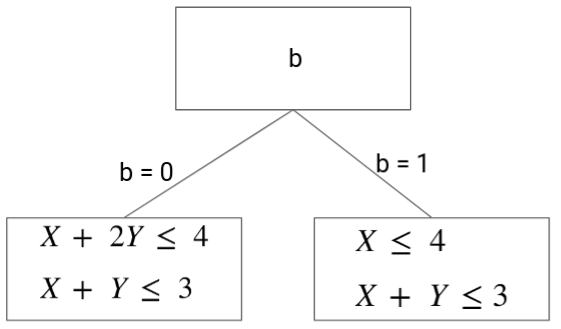
\includegraphics[scale=0.3]{Capitulos/Cap01_figs/branch-in-bound.png}
%     \caption{Arvore utilizada para realizar \textit{LP relaxation} e resolver individualmente os problemas de LP, ainda maximizando a equação \ref{eq:Cap01_MILP_Objective}.}
%     \label{fig:Cap01_TreeLP}
% \end{figure}
% Ao percorrer a arvore da figura \ref{fig:Cap01_TreeLP} resolvendo o LP comparando os resultados da equação \ref{eq:Cap01_MILP_Objective} e selecionando o melhor.
% \begin{itemize}
% \item
%   \textit{Web Service Description Language} \cite{wsdl:spec}: usada para
%     definir APIs que usam o protocolo SOAP. É uma linguagem baseada em XML.
%     Um exemplo de um arquivo WSDL é apresentado em \cref{anex:wsdl-example}.
% \item
%   \textit{OpenAPI} \cite{openapi:spec}: comumente usada para definir APIs que usam
%     o protocolo HTTP \cite{rfc2616}, informalmente chamadas de \textit{"Restful APIs"}
%     em referência ao conceito de REST definido em \cite{10.5555/932295}. É uma linguagem
%     baseada em YAML. Um exemplo de um arquivo OpenAPI é apresentado em \cref{anex:openapi-example}.
% \item
%   \textit{Protocol Buffers} \cite{googl:protobuf}: usada para definir APIs que usam
%     o protocolo gRPC \cite{googl:grpc}. O nome se refere tanto à IDL usada para a
%     especificação quanto para ao formato binário usado para transmitir as mensagens.
%     Um exemplo de um arquivo em Protocol Buffers é apresentado em \cref{anex:protobuf-example}.
% \end{itemize}

% Existem diversas vantagens em usar uma IDL, entre elas:

% \begin{enumerate}
% \item
%   A comunicação entre diferentes times (possivelmente em diferente organizações) que
%   precisam interagir via API é mais simples, já que todos os detalhes de interface
%   estão especificados em um formato padrão.
% \item
%   Pro esse motivo, é muito mais simples construir ferramentas de análise sobre a
%   especificação, como geradores de código, validadores, ferramentas de teste, etc.
% \end{enumerate}

\section{Algoritmo genético}

\cite{book:genetic_algo_data_structure}Algoritmos genéticos são algoritmos comumente utilizados para resolver problemas de otimização. 
Principalmente aqueles onde não podem ser equacionados, como certos problemas abstratos.
Estes não garantem uma solução ótima, mas com uma população suficientemente grande de genes e gerações pode-se reduzir as chances de erro ao menor possível.

Um algoritmo precisa ter essas características:
\begin{itemize}
\item
  Precisa possuir umas estrutura de dados que permite a fácil decodificação para uma combinação do resultado para o problema desejado, no caso do problema de empacotamento ela é convertida na posição dos objetos. Essas estruturas são chamadas de cromossomos e são comumente compostos por binários ou caracteres que são chamados de genes;
\item
  Criar a população inicial, onde o tamanho deve ser determinado pelos parâmetros;
\item
  Precisa de um método para avaliar a qualidade do cromossomo, como um sistema de score/fitness;
\item
  Um método de selecionar os cromossomos que originarão a população da próxima geração
\item
  Um método probabilístico de misturar conjuntos de genes da população vencedora. Pois estes conjuntos fazem parte de cromossomos que venceram diversas gerações, assim multiplicando bons conjuntos de genes através das gerações. Análogo ao que ocorre com a genética biológica. Este processo é chamado de cruzamento; 
\item
  Um método probabilístico de fazer pequenas alterações nos genes da próxima geração, assim gerando resultados próximos ao anterior, mas possivelmente melhores, assim é a caracterizado o processo de mutação.
\end{itemize}

\subsection{Estrutura de dados}
    No GA, a estrutura de dados que é utilizado para converter em informações do problema a ser resolvido é comumente chamado de cromossomo, que é um vetor de genes, onde estes são normalmente um bit, ou um caractere.

\begin{figure}[h]
    \centering
    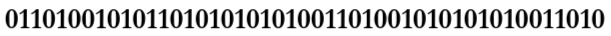
\includegraphics[scale=0.65]{Capitulos/Cap01_figs/genes_bit.png}
    \caption{Exemplo de uma gene onde os seus cromossomos são bits. Como a conversão desse gene se transforma em uma solução possível para o problema à ser resolvido, isso significa que para um gene de n bits, nos teremos $2^{n}$ soluções possíveis, fazendo a busca por força bruta ser impraticável para grandes valores de n.}
    \label{fig:Cap01_Genes_Bits_Example}
\end{figure}

\subsection{População de cromossomos}
É o conjunto de cromossomos, que são utilizados para possibilitar uma diversidade de genes desejada, que através da seleção, cruzamento e mutações apropriadamente calibradas, pode-se encontrar uma solução sub-ótima para o problema proposto.
\newline
Fatos a se ficar atento em uma população de genes é o risco da população começar a gerar respostas extremamente parecidas, fazendo o algoritmo ficar limitado em uma região de mínimo/máximo local. Fazendo-se necessária uma analise desse risco para a formulação dos algoritmos responsáveis pela geração seguinte.\newline

Outro fator que pode ser usado para acelerar a convergência para um bom resultado é a criação de uma população inicial bastante dispersa, aumentando as chances de diversos genes estarem próximos de pontos ótimos locais.\newline

\subsection{Avaliação}
Depois da decodificação de um cromossomo, se é feita uma função para quantificar a sua qualidade, assim permitindo comparação entre os cromossomos, consequentemente permitindo o processo de seleção, explicado na sub seção \ref{Cap_intro:sec_GA:sub_selection}.
\subsection{Seleção}\label{Cap_intro:sec_GA:sub_selection}
Pode-se desenvolver diversos algoritmos de seleção, onde um dos mais básicos e conhecidos é simplesmente escolher aleatoriamente dois cromossomos da população e o mais apto será copiado para compor a próxima geração, sendo este gene podendo ser selecionado múltiplas vezes, dessa forma a probabilidade de um conjunto de genes bons passar para a próxima geração aumenta.

\subsection{Cruzamento}
Devido ao fato dos cromossomos serem decodificados em dados para o problema desejado, dependendo como a estrutura dos genes é projetado, intervalos de genes de um cromossomo terão influencias no resultado de forma independente.\newline
Como exemplo: Pode-se pensar no caso do empacotamento, onde os cromossomos são divididos em intervalos iguais de genes, sendo que o primeiro intervalo representa a posição e rotação do primeiro objeto, o segundo intervalo representa o segundo objeto, seguindo essa logica até o fim.\newline
Ao termos genes compostos dessa forma, a população de genes pode possuir valores onde os cromossomos para objeto 2 do Cromossomo 1, melhoraria o Cromossomo 2. Fazendo-se desejável a formação de um novo cromossomo com os genes do segundo com os genes do objeto 2 do Cromossomo 1. Assim mostrando a relevância de cruzamento para o algoritmo genético.\newline
\begin{figure}[h]
    \centering
    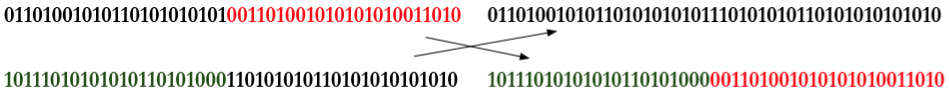
\includegraphics[scale=0.45]{Capitulos/Cap01_figs/cruzamento_pivot.png}
    \caption{Exemplo de um cruzamento de dois genes, onde ocorre a troca por entre as regiões delimitadas apenas por um pivô.}
    \label{fig:Cap01_cruzamento_pivot_Example}
\end{figure}
\newline
Apesar da figura \ref{fig:Cap01_cruzamento_pivot_Example} ser um cruzamento com o intervalo dos genes a serem cruzados delimitado por apenas um pivô, ou seja do pivô até o ultimo gene serão trocados. Pode-se fazer o cruzamento de outras formas, como num problema de empacotamento, é provavelmente mais interessante propor cruzamento com dois pivôs, onde um determina o primeiro e o outro o ultimo cromossomo trocado. Estes pivôs podem ser determinados de forma a tentar trocar os genes de objetos por inteiro ou parciais. Assim os melhores genes para um determinado objeto serão multiplicados com o passar das gerações.

\subsection{Mutação}
Com apenas os processos de seleção e cruzamento, o GA muito provavelmente ficaria preso em um ótimo local e sua população se tornaria muito parecida extremamente rápido. Dessa forma se faz necessário alterar os valores dos genes dos cromossomos de forma aleatória, mas não grosseira de forma que o cromossomo sofra poucas alterações de cada vez, assim garantindo uma diversidade a população e aumentando as probabilidades de se encontrar um valor de cromossomo melhor.

\subsection{Parâmetros}
 A escolha dos parâmetros é muito importante para um algoritmo genético, pois eles possuem grande influencia em como a população de genes de transforma ao passar da gerações, onde eles são definidos na lista abaixo da apostila \cite{algo_genetics_principios}:\newline
\begin{itemize}
\item
    Tamanho da População: Numero de espaço de busca sendo considerados em paralelo a cada ciclo
\item
    Taxa de \textit{crossover}: probabilidade(p\textunderscript{c}) de um individuo ser recombinado com outro(Cruzamento).
\item
    Taxa de mutação: probabilidade(p\textunderscript{m}) do conteúdo de uma posição/gene do cromossomo ser alterado.
\item
    Numero de gerações: Total de ciclos de uma evolução de um GA.
\item
    Total de indivíduos: total de tentativas em um experimento(tamanho da população x numero de gerações).
\end{itemize}

Sendo os dois últimos parâmetros são geralmente usados como critério de parada.

\section{Problemas}\label{cap:introducao:sec:problema}
Um dos problemas que serão propostos é inspirado em \textit{knolling}, que é uma tendência de estilo fotográfico onde se organizam objetos em uma figura de forma comumente retangular, mas ela pode ter múltiplas formas como no exemplo da figura \ref{fig:Cap01_Knolling_Photography_43}.
\begin{figure}[H]
    \centering
    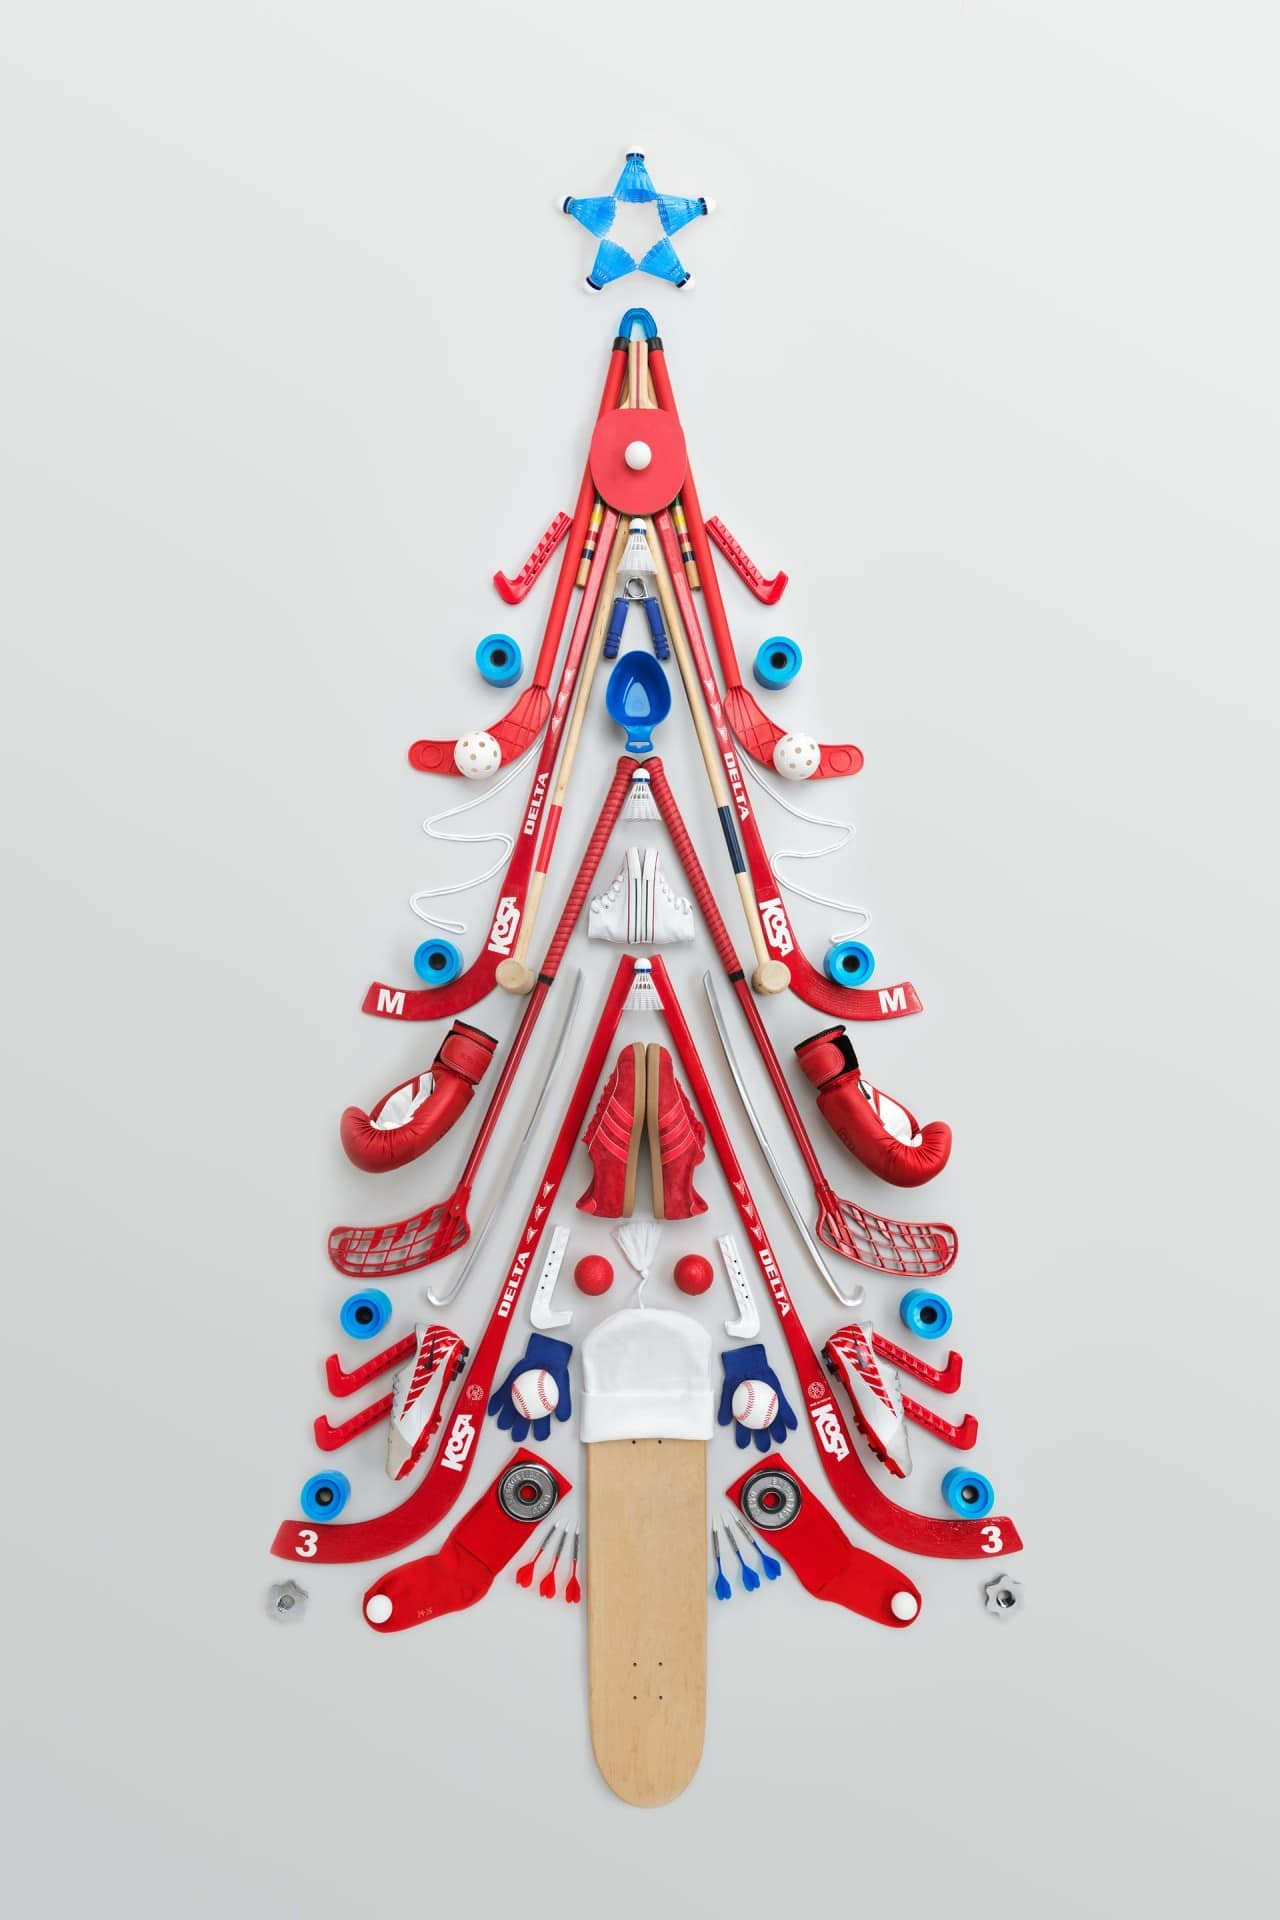
\includegraphics[scale=0.2]{Capitulos/Cap01_figs/Knolling-Photography-43.jpg}
    \caption{Exemplo de uma fotografia no estilo \textit{knolling} extraída de um site\cite{knolling:blog}. Onde se organiza os objetos formando uma figura alternativa.}
    \label{fig:Cap01_Knolling_Photography_43}
\end{figure}
Dessa forma serão proposto dois problemas à serem resolvidos por algoritmo genético:
\begin{enumerate}
\item
  Empacotar objetos tridimensionais num plano bidimensional de forma a obter um retângulo de menor área.
\item
  Empacotar objetos tridimensionais em um plano bidimensional dentro de uma região delimitada por uma forma geométrica, como está exemplificada na figura \ref{fig:Cap01_Knolling_Photography_43}. 
\end{enumerate}
% \begin{enumerate}
% \item
%   Como toda a parte dos modelos são geradas, servidor ou cliente, há uma significativa
%   redução no volume de linhas de código-fonte do sistema, reduzindo a possibilidade
%   de defeitos \cite{5010260} e facilitando o entendimento do projeto por novos
%   desenvolvedores.
% \item
%   Como o código é gerado a partir da especificação, sabemos que a implementação
%   vai estar de acordo com a interface especificada, permitindo que o programador
%   foque em implementar a lógica de cada operação, otimizando o uso do tempo. No
%   caso de consumidores, eles poupam o trabalho de ter que implementar um código
%   de integração com a API, que pode conter erros e ser difícil de manter,
%   principalmente com relação a mudanças e adições na API.
% \item
%   O código gerado abstrai toda a camada de comunicação e rede, tanto do servidor
%   quanto do cliente, facilitando o entendimento do código que o programador precisa
%   implementar.
% \end{enumerate}

% Existem diversos exemplos de geradores de APIs, alguns são \cite{openapi:gen} e
% \cite{googl:protobuf}.

% \section{ORMs}

% Da mesma forma que IDLs e geradores tentam facilitar o desenvolvimento da
% \textit{interface} de uma API, ORMs tentam facilitar a integração do código da
% API com o banco de dados usado (seja ele SQL ou NoSQL). Elas são bibliotecas que
% abstraem a execução de operações no banco de dados em uma interface amigável para
% a linguagem de programação usada. Por esse motivo, ORM é específica para a linguagem
% de programação em que ela foi implementada, e normalmente também é específica para
% um banco ou conjunto de bancos.

% ORMs normalmente funcionam via anotações e interfaces que o programador precisa
% adicionar ou implementar no código-fonte dos modelos. Essas anotações servem para,
% por exemplo, mapear o modelo a uma tabela, um campo a uma coluna, ou uma relação
% com outro modelo (1-1, 1-muitos ou muitos-muitos).

% Um exemplo em Python usando a ORM \texttt{sqlalchemy} é \cref{lst:sqlalchemy-example}.

% \begin{listing}[ht]
% \begin{minted}{python}
% from sqlalchemy import Column, DateTime, String, Integer, ForeignKey, func
% from sqlalchemy.orm import relationship, backref
% from sqlalchemy.ext.declarative import declarative_base


% Base = declarative_base()


% class Department(Base):
%     __tablename__ = 'department'
%     id = Column(Integer, primary_key=True)
%     name = Column(String)


% class Employee(Base):
%     __tablename__ = 'employee'
%     id = Column(Integer, primary_key=True)
%     name = Column(String)
%     # Use default=func.now() to set the default hiring time
%     # of an Employee to be the current time when an
%     # Employee record was created
%     hired_on = Column(DateTime, default=func.now())
%     department_id = Column(Integer, ForeignKey('department.id'))
%     # Use cascade='delete,all' to propagate the deletion of a Department
%     # onto its Employees
%     department = relationship(
%         Department,
%         backref=backref('employees',
%                          uselist=True,
%                          cascade='delete,all'))

% \end{minted}
% \caption{Exemplo de código usando \texttt{sqlalchemy}}
% \label{lst:sqlalchemy-example}
% \end{listing}

% ORMs são populares pois simplificam o trabalho do desenvolvedor ao automatizar muitas
% operações que são comumente realizadas no banco, e por prover uma DSL caso seja
% necessário fazer algo mais complexo. Dependendo da linguagem, essas funcionalidades
% podem ser validadas em tempo de compilação, previnindo defeitos.

% \section{Problema}

% Apesar de serem ferramentas muito populares, geradores de APIs e ORMs não integram
% bem. O primeiro costuma focar na \textit{interface de comunicação}, não prestando
% atenção a detalhes de implementação. Além disso, dado o grande número de ORMs
% presente para cada linguagem, e também as diversas formas de se gerar a interface
% de comunicação, geradores convencionais não conseguiriam adicionar suporte para
% todas as combinações possíveis.

% Outro problema em como os geradores são implementados hoje é que eles possuem
% suporte limitado a extensões externas ao código-fonte. Dependendo do gerador
% utilizado, é necessário implementar um \textit{novo gerador}, o que gera um grande
% custo operacional. Alguns exemplos de modificações possíveis:

% \begin{itemize}
% \item
%   Geração automática de testes para as operações \cite{9159071}.
% \item
%   Validação automática de propriedades das mensagens \cite{envoy:protoc-gen-validate}.
% \item
%   Integração com ORMs ou outras bibliotecas.
% \end{itemize}

% Devido a esses problemas, muitas organizações deixam de usar essas ferramentas e os
% programadores precisam implementar manualmente códigos que poderiam ser gerados.
% Isso aumenta a chance de erros ocorrerem durante a implementação, e o resultado divergir
% da especificação. Além disso, diminui a eficiência do time, pois há mais tarefas a
% serem realizadas.

% Avaliando as tarefas realizadas pelo time de engenharia de uma organização durante o
% ano de 2020, foi possível identificar que pelos menos 30\% das tarefas realizadas
% eram relacionadas a implementação de modelos, integração com ORMs e com a camada
% de comunicação da API. Além disso, dentro desses 30\%, ocorreram diversas vezes tarefas
% extras relacionadas com ajustes da implementação para que essa seguisse a especificação.

% Na tentativa de solucionar esse problema, esse trabalho propõe um novo modelo de
% gerador de APIs, que pode ser extendido para suportar qualquer linguagem ou funcionalidade
% nova sem a necessidade de modificar o código-fonte.

% Esse trabalho é estruturado como se segue. \cref{cap:past-works} faz uma análise
% de trabalhos anteriores. \cref{cap:proposal} apresenta, de forma detalhada, o que
% foi construído e a metodologia de análise.
